% How is it implemented?
% What technologies are used?
% General Architecture Overview

\section{Methodology}\label{sec:Methodology}
\subsection{Frontend}
Using a website as UI implementation has the benefits of being easy and fast to develop, accessible from nearly any device and wide support for backend technologies. The frontend uses the following tech-stack:
\begin{itemize}
    \item \textbf{React} as the frontend framework.
    \item \textbf{NextJS} for server-side rendering and routing.
    \item \textbf{TailwindCSS} for faster and more consistent styling.
    \item \textbf{NextUI} as component library.
\end{itemize}

The Website features 3 main pages:
\begin{itemize}
    \item \textbf{Weather} - A quick weather forecast for today and the next days.
    \item \textbf{Food Stock} - A list of food items labeled with their expiration date and storage location.
    \item \textbf{Todos} - Just a simple todo list for tasks of today.
\end{itemize}

\begin{figure}[H]
    \includegraphics[width=0.475\textwidth]{media/weather.png}
    \includegraphics[width=0.475\textwidth]{media/food.png}
    \includegraphics[width=0.475\textwidth]{media/todo.png}
    \caption{Website Pages}
    \label{fig:website}
\end{figure}

But before the user can access the website, they need to authenticate themselves. This is done by a simple login page, where a new user can register with email and password or a google login. After the user is authenticated, they are redirected to the main page and have data associated with their account.

\begin{figure}[H]
    \centering
    \includegraphics[width=0.475\textwidth]{media/login.png}
    \caption{Login Screen}
    \label{fig:login}
\end{figure}

\subsection{External APIs}
The website also features always changing background images, which are fetched from the Unsplash API. The images are fetched on the server-side and are cached for 1 hour. This way, the website always has a fresh look and feel. The free API has a limit of 50 requests per hour, which is more than enough for this project.

As for the weather forecast, the data is fetched from the OpenWeatherMap API. The API provides a simple and easy to use interface for the current weather and 5-day weather forecast with a bunch of extra sensor data, like humidity, pressure etc. available in the free tier.

\subsection{Backend}
The website is hosted on vercel under the url: \url{https://cds-dashboard.vercel.app/}.
Vercel provides an easy way to deploy NextJS applications, which are stored on a GitHub repository. The website is automatically deployed on every push to the main branch, which makes it ideal for a small project like this to get started quickly.

To store the user data, i.e. the food items and todos, a Supabase database is used. Supabase is an open-source Firebase alternative, which can also be self-hosted. There are other alternative for self-hosted databases, like MongoDB, or a simple SQL database, but Supabase comes with a lot of features out of the box, like authentication and a good API, reducing unecessary overhead.

To self-host the database, one must pull the docker image from the supabase github repository and run it.
Because Docker is creating a encapsulated environment, the database can be deployed to any machine running Docker, including a Raspberry Pi.
A Web Interface is provided by supabase, through which the database can be managed.
By importing a schema from a csv file, the schema is created automatically and can be adjusted to use authentication.

\begin{figure}[H]
    \centering
    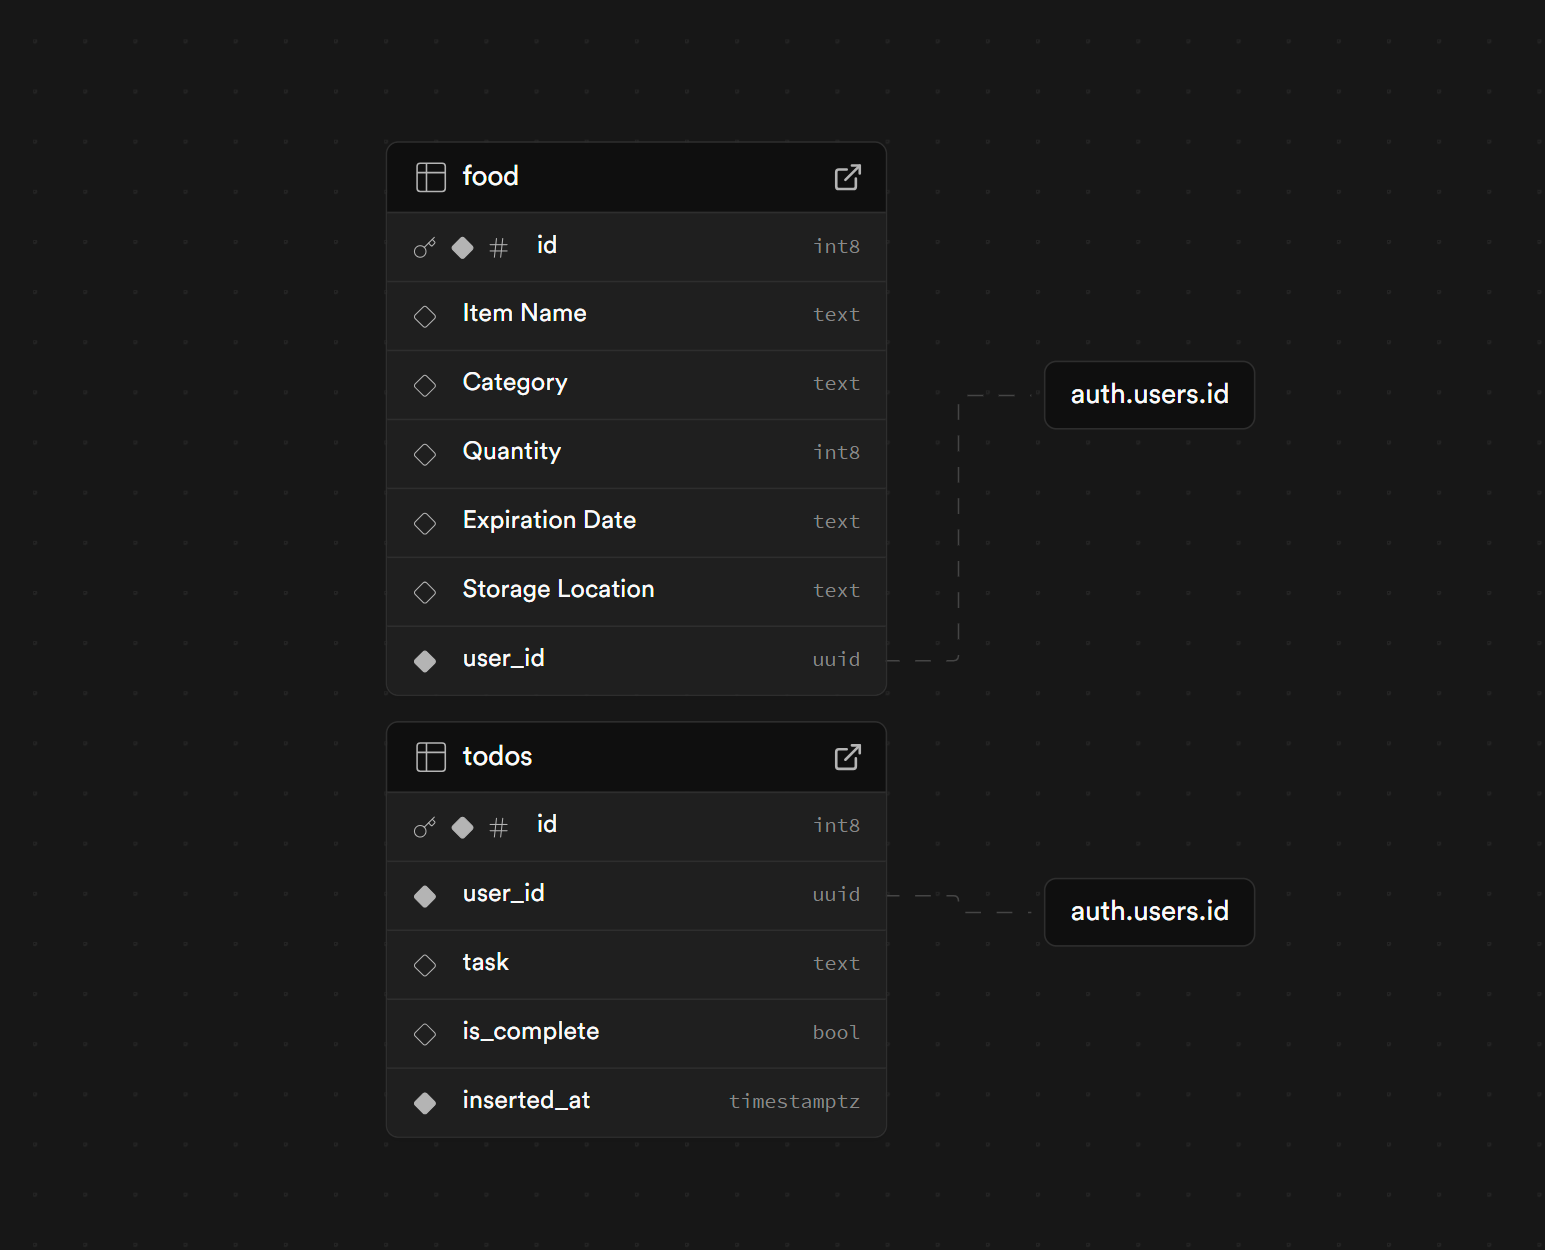
\includegraphics[width=0.475\textwidth]{media/database.png}
    \caption{Database Schema}
    \label{fig:schema}
\end{figure}

\subsection{Tunneling}
The only problem is that the Raspberry PI is only accessible from the local network. A solution to this would be to use port forwarding, but this requires a static IP address, a lot of configuration and is not very secure for a home network. A better solution is to use a tunneling service like ngrok. Ngrok creates a secure tunnel to the Raspberry PI, which can be accessed from anywhere in the world.
To implement this, it is as easy as to install the ngrok package on the Raspberry PI, login to your account and run the command \texttt{ngrok http 3000}. Only the Supabase URL in the Google Cloud and frontend configuration need to be replaced with the ngrok URL, following this change.
